\documentclass[a4paper, 12pt, twoside]{book}

\usepackage{graphicx}
\usepackage{geometry}
\geometry{a4paper,top=2cm,bottom=2cm,left=2cm,right=2cm, headheight=15pt,bindingoffset=5mm}
\usepackage{floatflt}
\usepackage{amssymb}
\usepackage{epstopdf}
\usepackage{color}
\usepackage{booktabs}
\usepackage[english]{babel}
\usepackage{setspace}
\usepackage{amscd}
\usepackage[T1]{fontenc}
\usepackage[utf8]{inputenc}
\usepackage{cancel}
\usepackage{float}
\usepackage{longtable}
\usepackage{multirow}
\usepackage{pdflscape}
\usepackage{eurosym}
\usepackage{amsmath}
\usepackage{mathcomp}
\usepackage{rotating}
\usepackage{pdfpages}
\usepackage[parfill]{parskip}
\usepackage[a-1b]{pdfx}
\usepackage{hyperref}
\usepackage{varioref}
\usepackage{cleveref}
\usepackage{tocbibind}
\usepackage[autostyle]{csquotes}
%\usepackage{tabto}
\usepackage{enumitem}
\usepackage{setspace}
\usepackage{lmodern}


%%% appendix
\usepackage[toc,page]{appendix}

%%% bibliography
\usepackage[backend=biber,giveninits=true,sorting=nty,maxcitenames=1,style=numeric ,uniquelist=false, uniquename=false]{biblatex}

\setlength\bibitemsep{\baselineskip}

\addbibresource{bibThesis.bib}
\usepackage{fancyhdr}
\usepackage[format=hang,labelfont=bf,font=small,tableposition=top]{caption}
\renewcommand\textfraction{.05}
\hypersetup{
%     		pdfa,
			%bookmarks=true,
			%
			%hyperfootnotes=false,
			colorlinks=true,
			linkcolor=black,
			anchorcolor=black,
			citecolor=blue,
			urlcolor=black,
			%pdftitle={Bachelor Thesis},
			%pdfauthor={Sabrina Ciccolo},
}
\DeclareGraphicsRule{.tif}{.png}{.png}{`convert #1 `dirname #1`/`basename #1 .tif`.png}
\pagestyle{plain}

\newcommand{\citev}[1]{\citeauthor{#1} \citeyear{#1} \cite{#1}}

\setlength{\parindent}{0pt}
\setcounter{secnumdepth}{3}
\setcounter{tocdepth}{3}

%------------------------------------------%
%--------------- TITLE PAGE ---------------%
%------------------------------------------%

\title{Cross-View Association of Identical Parts Across Non-Overlapping 3D Scans: Identifiability, Shift Ambiguity and Evaluation}
\author{Sabrina Ciccolo}

\begin{document}

\begin{titlepage}

\newgeometry{top=2cm,bottom=2cm,left=2cm,right=2cm, heightrounded,bindingoffset=0mm}

\begin{center}

\begin{figure}[h]
\centering

\includegraphics[width=4cm]{fig/units.png}
\end{figure}

\vspace{1cm}

\Large
UNIVERSITY OF TRIESTE

\vspace{0.25cm}

\Large
Department of Mathematics, Informatics and Geosciences

\vspace{0.5cm}

\Large
Bachelor's Degree in Artificial Intelligence and Data Analytics

\vspace{0.75cm}

\hrule

\vspace{0.25cm}
\normalsize


\vspace{2cm}
\large
BACHELOR'S THESIS


\vspace{1.15cm}

\begin{spacing}{1.25}
{\bf \fontsize{16}{20}\selectfont Cross-View Association of Identical Parts Across Non-Overlapping 3D Scans: Identifiability,\\ Shift Ambiguity and Evaluation\par}
\end{spacing}

\vspace{4.5cm}

\end{center}

\hspace{.05\textwidth}
\begin{minipage}[c]{.52\textwidth}
\begin{flushleft}
\large
\textit{Supervisor: }\\
Prof. Alejandro Rodriguez Garcia
\end{flushleft}
\end{minipage}
\hspace{0.12\textwidth}%
\begin{minipage}[c]{.23\textwidth}
\begin{flushleft}
\large
\textit{Candidate: }\\
Sabrina Ciccolo\\
\end{flushleft}
\end{minipage}

\vspace{1.5cm}

\hrule

\vspace{0.25cm}

\begin{center}
\large
\textit{Academic Year }2025/2026
\end{center}

\end{titlepage}

\restoregeometry
\normalsize

\clearpage
\null
\thispagestyle{empty}
\clearpage

%------------------------------------------%
%---------------- ABSTRACT ----------------%
%------------------------------------------%

\frontmatter
\clearpage
\null
\clearpage

%------------------------------------------%
%---------------- CONTENTS ----------------%
%------------------------------------------%

{\fontsize{12}{18}\selectfont\tableofcontents\par}
{\fontsize{12}{18}\selectfont\listoffigures\par}
{\fontsize{12}{18}\selectfont\listoftables\par}

\clearpage
\null
\clearpage

%------------------------------------------%
%---------------- CHAPTERS ----------------%
%------------------------------------------%

\newpage
\mainmatter
\pagestyle{fancy}
\fancyhead[L,R]{}
\fancyhead[C]{\nouppercase{\leftmark}}


\chapter{Introduction}
\label{ch:intro}

\section{The problem}
\label{sec:intro-problem}

Industrial handling is increasingly automated. Repetitive and heavy tasks such as lifting or sorting parts, once assigned to human operators, are now delegated to robots to satisfy the cycle time required by the production line.

For a robot to grasp an object, it is necessary to determine the object's pose, which dedicated sensors measure as a position and an orientation relative to the robot's own coordinate frame.

For a single compact piece, one 3D sensor is usually sufficient, as its viewpoint can cover the entire object. On the other hand, a very long part cannot be captured from a single viewpoint, making a single scanner insufficient. The layout therefore requires two sensors, one for each end. The part is gripped precisely at these ends, whose faces also determine the 6D pose of a straight extruded profile up to the symmetry of the cross-section.

The setup consists of two structured-light 3D scanners, positioned at either end of a conveyor carrying bundles of six-metre metal bars of identical profile.

Each device is mounted on a dedicated carriage at one end of the bundle, facing the end faces of the bars rather than their length. The two carriages are separated by several metres along the axis of the bar. The part of the bundle that each scanner covers is often narrower than the bundle itself, so a single view does not always contain every bar. Because the two sensors face opposite ends, their respective viewpoints neither overlap nor capture any common surface. Finally, a dual-arm manipulator picks up each bar by gripping it at both ends. \Cref{fig:rig} illustrates this setup.

\begin{figure}[htbp]
\centering
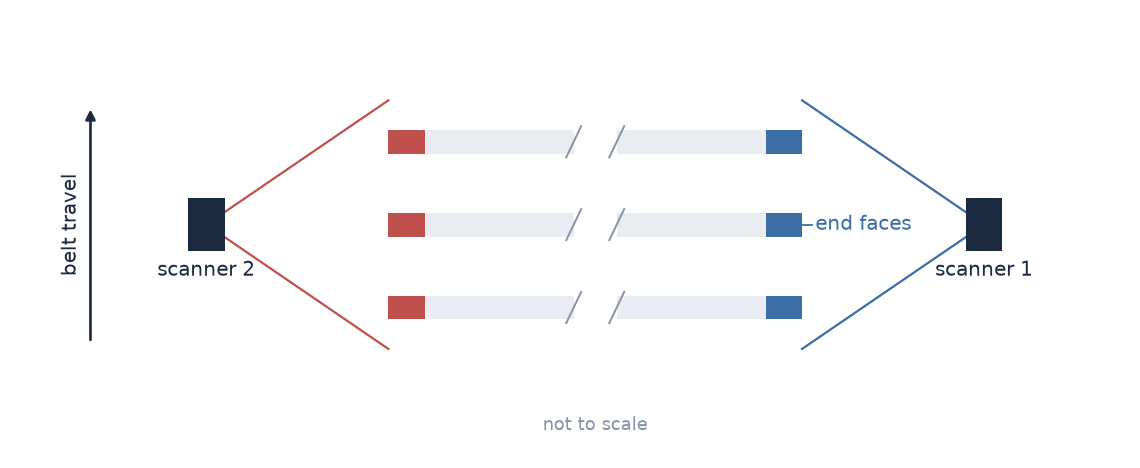
\includegraphics[width=\textwidth]{fig/f1_rig.png}
\caption[Dual-scanner system]{Dual-scanner system. Top view of the system. Each scanner is positioned at one end of the bundle and detects only the end faces of the bars facing it. In the figure, these faces are highlighted at both ends of each bar. The viewpoints of the two scanners do not share any surface and the bundle passes through both. Neither axis is to scale.}
\label{fig:rig}
\end{figure}



%------------------------------------------%
%-------------- BIBLIOGRAPHY --------------%
%------------------------------------------%

\cleardoublepage
\pagestyle{plain}
{
\backmatter
\phantomsection
\addcontentsline{toc}{chapter}{\bibname}


%\nocite{*}

\AtNextBibliography{\small}
\sloppy
\printbibliography
}

\end{document}
